%% Le lingue utilizzate, che verranno passate come opzioni al pacchetto babel. Come sempre, l'ultima indicata sar� quella primaria.
%% Se si utilizzano una o pi� lingue diverse da "italian" o "english", leggere le istruzioni in fondo.
\def\thudbabelopt{english,italian}
%% Valori ammessi per target: bach (tesi triennale), mst (tesi magistrale), phd (tesi di dottorato).
\documentclass[target=mst]{thud}[2014/03/11]

%% Aggiunta pacchetto per inserimento di immagini
\usepackage{graphicx}
\graphicspath{ {img/Introduzione/} {img/ContestoTecnologico/1_PCNEurotech/} }

%% --- Informazioni sulla tesi ---
%% Per tutti i tipi di tesi
\title{Elaborazione di Immagini in ambito Embedded con OpenCV: Passenger Counter}
\author{Mattia Dal Ben}
\course{Ingegneria Elettronica}
\supervisor{Prof.\ Antonio Abramo}
\cosupervisor{Ing.\ Marco Carrer}
%% Altri campi disponibili: \reviewer, \tutor, \chair, \date (anno accademico, calcolato in automatico).
%% Con \supervisor, \cosupervisor, \reviewer e \tutor si possono indicare pi� nomi separati da \and.
%% Per le sole tesi di dottorato
\phdnumber{313}
\cycle{XXVIII}
\contacts{Via della Sintassi Astratta, 0/1\\65536 Gigatera --- Italia\\+39 0123 456789\\\texttt{http://www.example.com}\\\texttt{inbox@example.com}}
\rights{Tutti i diritti riservati a me stesso e basta.}
%% Campi obbligatori: \title, \author e \course.

%% --- Pacchetti consigliati ---
%% hyperref: Regola le impostazioni della creazione del PDF... pi� tante altre cose.
%% tocbibind: Inserisce nell'indice anche la lista delle figure, la bibliografia, ecc.

%% --- Stili di pagina disponibili (comando \pagestyle) ---
%% sfbig (predefinito): Apertura delle parti e dei capitoli col numero grande; titoli delle parti e dei capitoli e intestazioni di pagina in sans serif.
%% big: Come "sfbig", solo serif.
%% plain: Apertura delle parti e dei capitoli tradizionali di LaTeX; intestazioni di pagina come "big".

\begin{document}

%% Il frontespizio prima di tutto!
\maketitle

%% Dedica (opzionale)
%% \begin{dedication}A mia madre.\end{dedication}

%% Ringraziamenti (opzionali)
%% \acknowledgements
%% Sed vel lorem a arcu faucibus aliquet eu semper tortor. Aliquam dolor lacus, semper vitae ligula sed, blandit iaculis leo. Nam pharetra lobortis leo nec auctor. Pellentesque habitant morbi tristique senectus et netus et malesuada fames ac turpis egestas. Fusce ac risus pulvinar, congue eros non, interdum metus. Mauris tincidunt neque et aliquam imperdiet. Aenean ac tellus id nibh pellentesque pulvinar ut eu lacus. Proin tempor facilisis tortor, et hendrerit purus commodo laoreet. Quisque sed augue id ligula consectetur adipiscing. Vestibulum libero metus, lacinia ac vestibulum eu, varius non arcu. Nam et gravida velit.

%% Sommario (opzionale)
\abstract
Nello sviluppo di questa tesi si \`e affrontato lo studio e la progettazione di un sistema di conteggio dei passeggeri su una piattaforma embedded. Il software applicativo \`e basato su algoritmi di elaborazione di immagine resi disponibili dalla libreria open-source per l'image processing OpenCV. La piattaforma software \`e stata realizzata utilizzando il progetto Yocto, il quale permette la creazione di distribuzioni Linux customizzate e targettate all'utilizzo in abito embedded.
L'applicazione di Passenger Counter ha come scopo quello di contare i passeggeri che attraversano in entrata e in uscita le porte di un mezzo pubblico, in modo tale da permettere un conteggio esatto delle persone presenti sul mezzo.
Lo sviluppo si \`e diviso in quattro fasi principali:
\begin{itemize}
\item Una indagine preliminare sulle migliori piattaforme sulle quali sviluppare l'applicazione.
\item Progettazione e implementazione del contatore usando solamente algoritmi di elaborazione delle immagini (Passenger Counter con background subtraction), individuando i passaggi pi\`u pesanti dal punto di vista computazionale.
\item Progettazione e implementazione del contatore sfruttando telecamere a infrarossi Time-Of-Flight (Passenger counter con telecamere RealSense).
\item Lo sviluppo della piattaforma software sulla quale integrare tutte le tecnologie utilizzate in fase di sviluppo per mezzo del progetto Yocto.
\end{itemize}

%% Indice
\tableofcontents

%% Lista delle tabelle (se presenti)
%\listoftables

%% Lista delle figure (se presenti)
\listoffigures

%% Corpo principale del documento
\mainmatter

%% Parte
%% La suddivisione in parti � opzionale; talvolta sono sufficienti i capitoli.
%% \part{Parte}

%% Capitolo 1: Introduzione
\chapter{Introduzione}
Nel seguito viene riportato il contesto all'interno del quale si configura l'applicazione sviluppata nel corso della tesi. Quindi verr\`a descritto l'applicazione del Passenger Counter e gli obiettivi di questa tesi. Nel secondo capitolo verr\`a affrontato il contesto tecnologico di dettaglio mentre nel terzo capitolo verr\`a trattata la realizzazione vera e propria dell'applicazione. 

%% Sezione Contesto IoT
%% NOTA: L'intera sezione che segue \`e stata presa dalla Wikipedia inglese alla voce: Internet of Things.
\section{Il contesto IoT}
L'Internet of Things (IoT) \`e l'internconnesione di device, veicoli, edifici e oggetti dotati di elettronica, software, sensori, attuatori e connettivit\`a che permettono a questi oggetti di raccogliere e scambiare dati. L'IoT permette agli oggetti di essere rilevati e controllati in remoto attraverso l'infrastruttura di rete esistente, creando opportunit\`a per una integrazione pi\`u diretta del mondo fisico all'interno di sistemi informatizzati, con l'obbiettivo di aumentare l'efficienza, la precisione e il beneficio economico riducendo al contempo la necesssit\`a dell'intervento umano. Tipicamente ci si aspetta che l'IoT offra connettivit\`a avanzata tra device, sistemi e servizi che vadano oltre la comunicazione Machine-to-machine (M2M) e coprano una variet\`a di protocolli, domini ed applicazioni. L'obiettivo \`e quello di introdurre processi di automazione in tutti i settori.

%% Storia dell'IoT
\subsection{Storia dell'Internet of Things}
Il neologismo inglese Internet of Things \`e stato introdotto per la prima volta da Kevin Ashton, cofondatore e direttore esecutivo di Auto-ID Center (consorzio di ricerca con sede al MIT), durante una presentazione nel 1999, ma il concetto di una rete di device "intelligenti" fu discusso per la prima volta nel 1982, con un distributore di bibite opportunamente modificato per interfacciarsi ad internet dalla Carniegie Mellon University. Esso era capace di riportare il suo inventario e qualora le bibite di cui era appena stato rifornito fossero ancora calde. Tra il 1993 e il 1996 molte aziende cominciarono a proporre soluzioni per l'Internet delle Cose ma \`e solamente dopo il 1999 che il settore cominci\`o ad assumere rilevanza. Le prime applicazioni per questo tipo di concetti erano l'inventariamento degli oggetti all'interno di fabbriche. Ci\`o poteva essere realizzato utilizzando tag RFID (Radio-frequency Identification) che permettessero ai sistemi informatici di identificare e tracciare gli oggetti presenti all'interno di ambienti vasti. Questo tipo di applicazione dell'IoT \`e ormai pratica standard nota come RFID Asset Tracking.
Ad oggi il concetto di IoT si \`e molto evoluto grazie al progresso tecnologico. La capacit\`a di integrare negli oggetti elettronica, sensori e connettivit\`a wireless ne ha ampliato le capacit\`a e le possibili applicazioni. Nel settore IoT ora convergono molteplici tencologie quali real-time analytics, machine learning, commodity sensors e sistemi embedded.

%% Parte di questa sezione l'ho rubacchiata da wikipedia cercando: Industria 4.0
\subsection{Sviluppi futuri}
\begin{figure}[h!]
  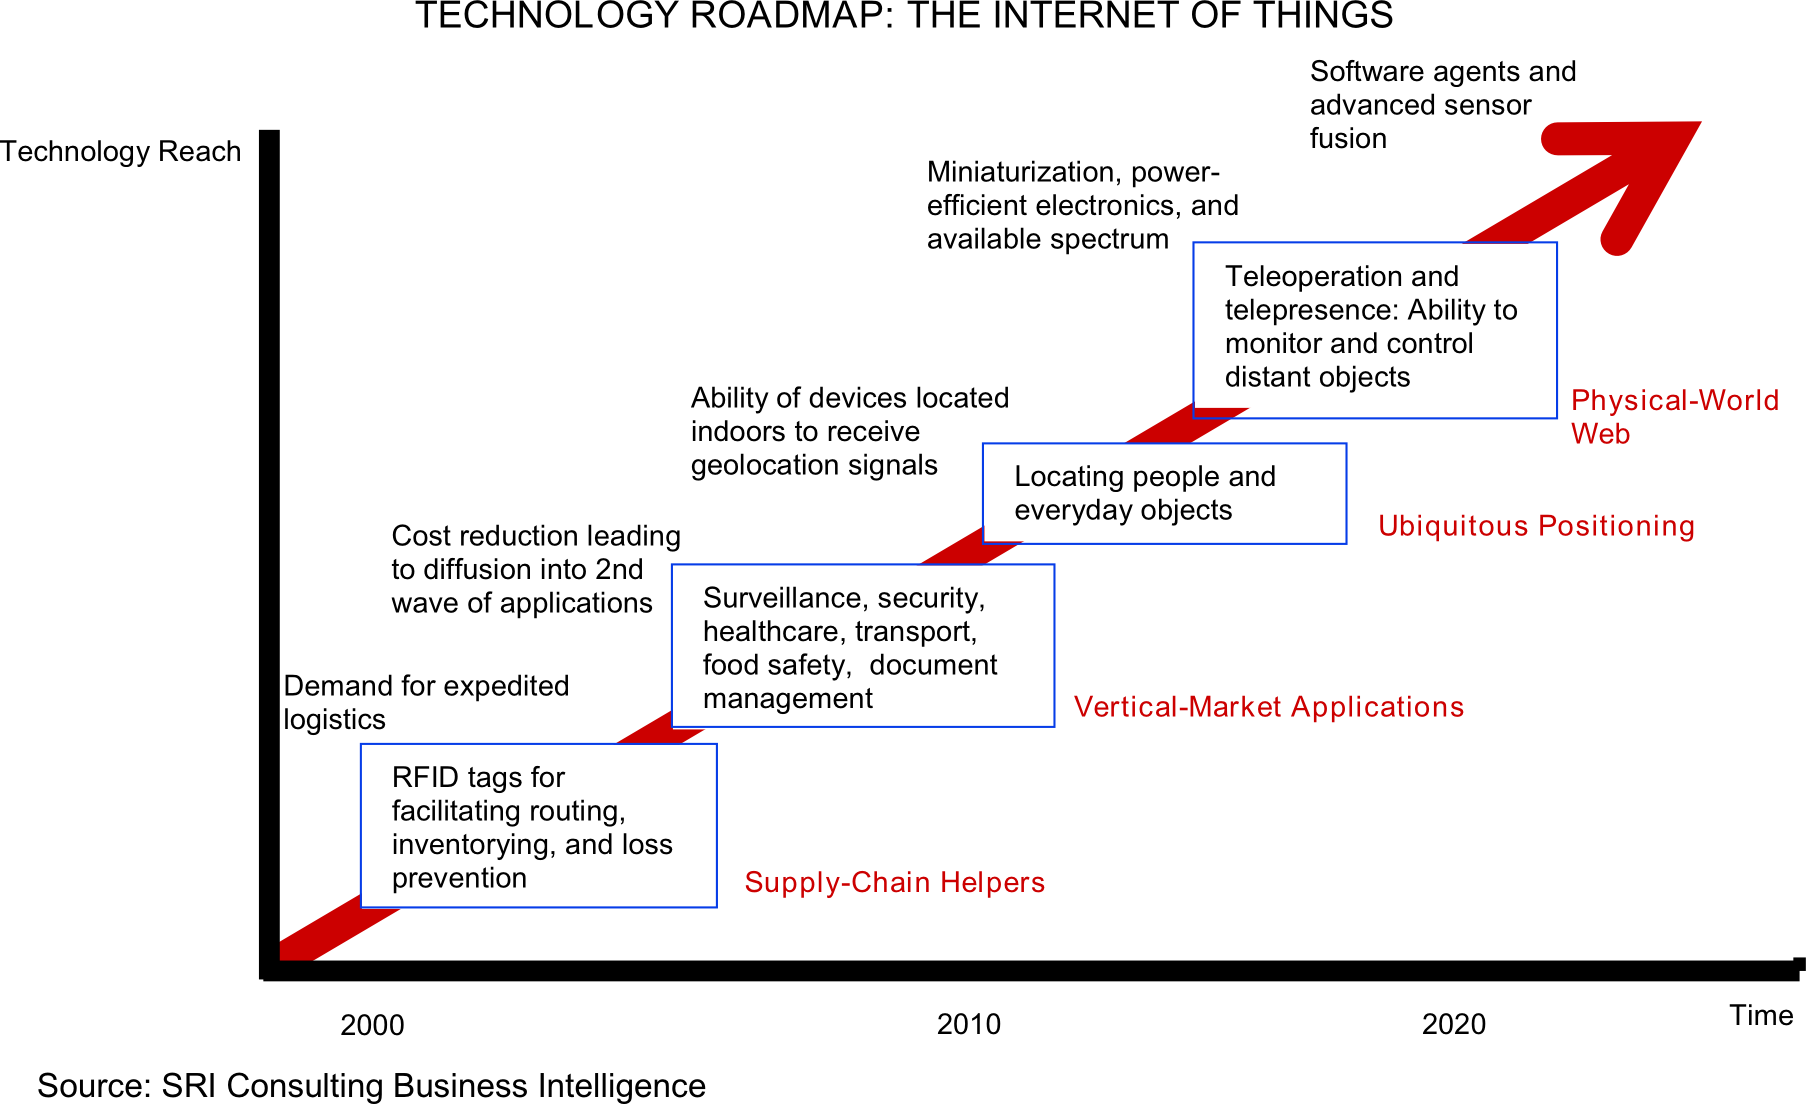
\includegraphics[width=\linewidth]{Internet_of_Things.png}
  \caption{Trend dell'internet of things}
  \centering
  \label{fig:trendIoT}
\end{figure}
Secondo le proiezioni di Gartner, Inc. una corporation per la ricerca e advisory tecnologica, entro il 2020 ci saranno oltre 20 miliardi di device connesse all'Internet of Things. Si sta parlando di una Industria 4.0 dove l'automazione industriale integra l'IoT per migliorare le condizioni di lavoro e la produttivit\`a. La chiave di volta dell'Industria 4.0 sono i sistemi ciberfisici (CPS), ovvero sistemi fisici che sono strettamente connessi con i sistemi informatici e possono interagire e collaborare con altri sistemi CPS i quali costituiscono lo step evolutivo successivo delle device IoT. 
Un altro settore nel quale si proiettano ulteriori sviluppi \`e la Big Data Analysis. L'ubiquit\`a dei dispositivi intelligenti connessi all'Internet delle Cose permette analisi di dati vastissimi ai quali precedentemente era impensabile avere accesso. Le informazioni che si possono ricavare da questi dati sono molteplici e di sicuro interesse per molti ambiti di applicazione.

%% Interruzione di pagina
\newpage

%% Classi di applicazioni IoT
\section{Classi di applicazioni IoT}
Passiamo ora ad analizzare i campi di applicazione pi\`u diffusi per l'Internet delle Cose.

%% Qui ho rubato da Wikipedia inglese il paragrafo sulle Applications nella pagina dedicata all'IoT
\subsection{Environmental monitoring}
Le applicazioni di monitoraggio ambientale tipicamente utilizzano sensori collegati all'Internet delle Cose per fornire assistenza nella protezione dell'ambiente. Il monitoraggio pu\`o interessare la qualit\`a dell'aria o dell'acqua, condizioni atmosferiche o del suolo, e pu\`o includere aree come il monitoraggio degli spostamenti della fauna selvatica e del suo habitat. Ci\`o pu\`o avere applicazioni anche nell'ambito della rilevazione di disastri naturali: sistemi di allerta per terremoti e tsunami possono essere implementati nell'ambito IoT. Device IoT in questo campo di applicazione sono tipicamente dislocate su un'ampia area geografica possono anche essere mobili.

\subsection{Infrastructure management}
Il monitoraggio e il controllo di infrastrutture urbane come ponti, rotaie, wind-farms \`e un campo di applicazione chiave dell'IoT. L'infrastruttura IoT pu\`o essere usata per monitorare eventi o cambiamenti nelle condizioni strutturali che possono compromettere la sicurezza o aumentare i rischi. Pu\`o altres\`\i\ essere usato per la programmazione di interventi di manutenzione in maniera pi\`u efficiente coordinando le operazioni tra diversi fornitori di servizi. Le device IoT sono anche usate per controllare infrastrutture critiche come ponti per fornire accesso alle navi. Si pensa che l'utilizzo di device IoT possa migliorare la gestione degli incidenti e la coordinazione in caso emergenze, la qualit\`a del servizia e ridurre i costi in tutte le aree legate alla gestione delle infrastrutture.

\subsection{Manufacturing}
L'ambiente manifatturiero \`e sicuramente una delle applicazioni di punta dell'IoT fina dalla sua nascita. Gli inteventi dell'IoT spaziano dalla gestione degli equipaggiamenti al tracking degli asset nell'ambiente produttivo. Questa sinergia permette alle aziende di avere una maggior flessibilit\`a e di ottimizzare in tempo reale i sistemi di produzione nonch\`e la rete di approviggionamento grazie all'interconnesione tra macchinari, sensori e sistemi.
L'integrazione di sistemi IoT all'interno di catene di produzione permette la predictive maintenance, valutazione statistica della degradazione dello stato dei macchinari, e prevenzione di guasti.
Come visto in precedenza l'evoluzione dell'Industria 4.0 \`e interamente basata sull'integrazione tra sistemi di produzione e l'Internet of Things.

\subsection{Energy management}
L'intregrazione di reti di sensori e attutatori, connessi ad internet, si pensa possa ottimizzare il consumo energetico in ambito industriale e casalingo. L'integrazione di device IoT all'interno di contatori per l'energia, cos\`\i\ come dispositivi domestici e industriali, capaci di comunicare con le compagnie per la rete elettrica possono permettere una gestione migliore della generazione ed utilizzo dell'energia. Questo tipo di device inoltre permetterebbe agli utenti di controllare in remoto i loro dispositivi, o controllarli centralmente grazie a interfacce cloud, in modo tale da implementare funzioni avanzate come la programmazione delle accensioni o dell'utilizzo dei dispositivi. Questo tipo di applicazioni \`e molto diffuso nel campo della domotica, i termostati IoT sono un ottimo esempio di questa applicazione.

\subsection{Medical and Healthcare}
Device connesse all'Internet delle cose possono essere abilitare il monitoraggio remoto dello stato di salute e sistemi di notifica delle emergenze. Queste device per il rilevamento dello stato di salute possono variare dal rilevamento della pressione arteriosa fino al conteggio dei battiti del cuore. Alcuni ospedali hanno cominciato ad utilizzare "letti smart" in grado di rilevare quanto il letto \`e occupato e quando il paziente sta cercando di alzarsi. Ormai sono molto diffusi dispositivi per il tracciamento delle attivit\`a dell'utente che incoraggiano uno stile di vita salutare, in questo ambito rientrano le wearable device come i fitness trackers.

\subsection{Settore dei trasporti}
%% Qui mi ricollego al PCN che \`e la sezione seguente
L'IoT pu\`o dare assistenza nella integrazione delle comunicazioni, controlli e elaborazione delle informazioni attraverso vari sistemi di trasporto. Le applicazioni dell'IoT si estendono a tutti gli aspetti dei sistemi di trasporto: i veicoli, l'infrastruttura, il pilota e i passeggeri. L'interazione dinamica tra questi componenti permette una comunicazione inter e intra veicolare, controllo del traffico intelligente, smart parking, gestione della logistica e delle flotte, controllo dei veicoli e sicurezza stradale.
L'applicazione sviluppata nel corso della tesi \`e appunto legata a questo ambito di applicazione dell'IoT e nel prossimo paragrafo ne analizzeremo gli obiettivi e funzionalit\`a.

%% Interruzione di pagina
\newpage

%% Sezione PCN
\section{Passenger Counter}
Passiamo ora a contestualizzare il lavoro svolto per questa tesi all'interno dell'ambito IoT.

Il Passenger Counter, o contatore di passeggeri, \`e un dispositivo IoT la cui funzione \`e quella di rilevare e conteggiare i passeggeri presenti all'interno di un sistema di trasporto pubblico. Esso deve altres\`\i\ fornire i dati in tempo reale al fornitore dei servizi sfruttando l'Internet delle Cose in modo tale da permettere una gestione pi\`u efficiente della flotta dei mezzi di trasporto. Il dispositivo deve essere in grado di effettuare il conteggio in modo non invasivo e contact-less, tenendo conto delle restrizioni dovute all'ambiente nel quale deve essere applicato.

\begin{figure}[h!]
  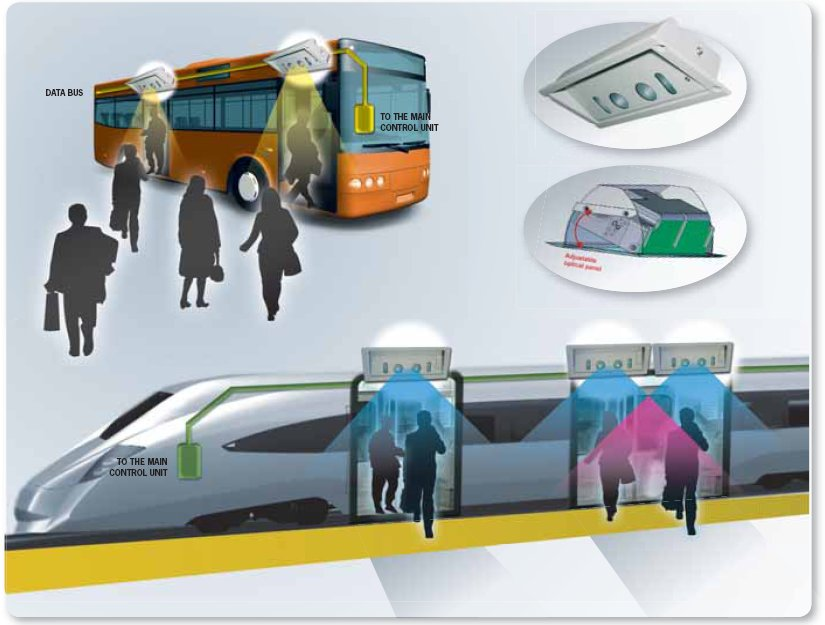
\includegraphics[width=9cm]{PassengerCountersz.jpg}
  \centering
  \caption{Schematizzazione del contatore di passeggeri}
  \label{fig:SchemPCN}
\end{figure}

Il lavoro presentato in questa tesi \`e stato commissionato da Eurotech: azienda dedicata alla ricerca, sviluppo e produzione di sistemi embedded e computer ad alte prestazioni e con sede ad Amaro. L'azienda inoltre ha una forte rilevanza in ambito IoT in quanto, oltre a fornire dispositivi IoT ready, ha realizzato una piattaforma Machine-to-Machine che consente ai dispositivi, ai sensori e a tutti i sistemi distribuiti sul campo di comunicare tra loro trasferendo le informazioni rilevanti alle business application ed alle infrastrutture IT. Il PCN o Passenger Counter \`e uno dei prodotti di punta dell'azienda ed \`e stato selezionato come progetto per questa tesi.

\begin{figure}[h!]
  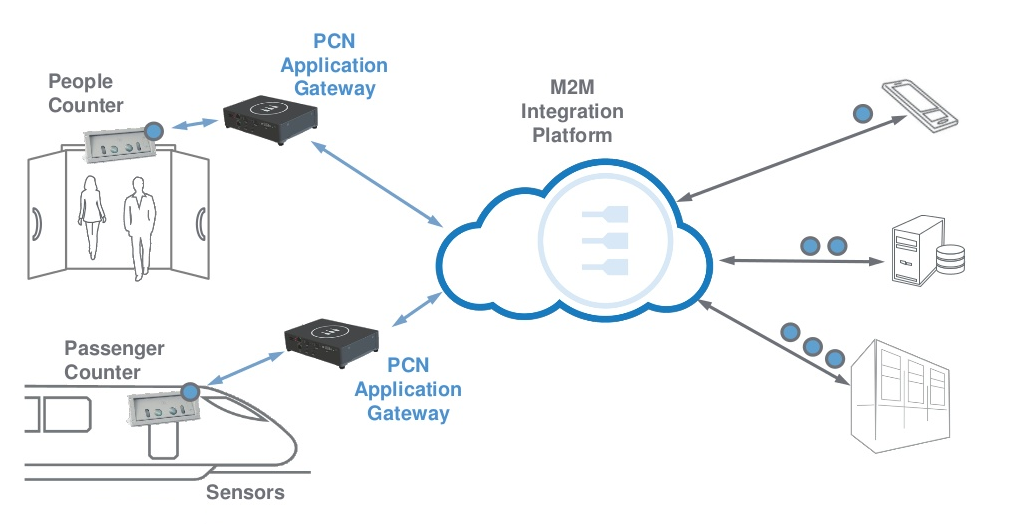
\includegraphics[width=\textwidth]{SchemaPCNIoT.png}
  \centering
  \caption{Schema Passenger Counter Eurotech}
  \label{fig:SchemPCNEurotech}
\end{figure}

Il sistema di conteggio di passeggeri consta di tre parti fondamentali come schematizzato in figura \ref{fig:SchemPCNEurotech}:
\begin{enumerate}
\item Dispositivo di acquisizione video.
\item Dispositivo di elaborazione e trasmissione dei dati in real-time.
\item Infrastruttura di rete cloud per il raccoglimento dei dati.
\end{enumerate}
\`E quindi possibile accedere ai dati raccolti da pi\`u dispositivi per mezzo della piattaforma M2M proprietaria di Eurotech.

\section{Obiettivi della tesi}
L'obiettivo della tesi \`e stato quello di realizzare una nuova versione del Passenger Counter di Eurotech basandosi sulla infrastruttura software/hardware fornita dall'azienda, cercando di migliorare quanto gi\`a fatto da Eurotech, esplorando soluzioni tecnologiche alternative. Questo obiettivo \`e stato quindi suddiviso in tre parti:
\begin{enumerate}
\item Identificare gli ambienti di sviluppo pi\`u idonei alla realizzazione del progetto.
\item Realizzare una nuova versione del Passenger Counter puntando a migliorare le prestazione ed abbattere i costi, adattandolo alle tecnologie usate dall'azienda per i suoi prodotti. 
\item Realizzare una infrastruttura software che fornisse tutti gli strumenti e le librerie necessarie all'implementazione del Passenger Counter realizzato e che potesse essere installato sulla piattaforma hardware fornita da Eurotech.
\end{enumerate}

%% Capitolo 2: Contesto tecnologico di dettaglio
\chapter{Contesto tecnologico di dettaglio}
Passiamo ora a descrivere pi\`u tecnicamente e nel dettaglio le tecnologie utilizzare nello svolgimento della tesi.

\section{Tecnologie PCN Eurotech}

\begin{figure}[h!]
  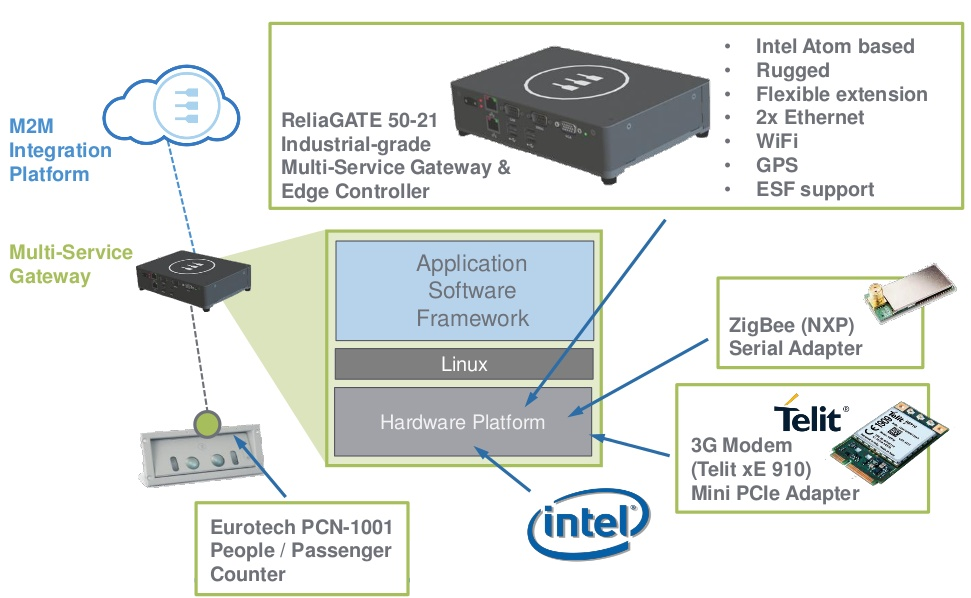
\includegraphics[width=\textwidth]{StrutturaPCN.png}
  \centering
  \caption{Struttura del Passenger Counter di Eurotech}
  \label{fig:PCNEurotechHardware}
\end{figure}

\subsection{Hardware}
Il sistema di conteggio dei passeggeri consta di due componenti hardware fondamentali: il gateway e il dispositivo di acquisizione delle immagini.

Il gateway \`e un'altro prodotto della Eurotech noto come ReliGATE 50-21. Utilizza un processore x86 Intel Atom Z510P al quale sono state aggiunte opportune interfacce di rete per il deployment mobile. Esso ha infatti interfacce 2G/3G, WiFi, 802.15.4/Zigbee e GPS. Questo componente rappresenta l'unit\`a di elaborazione centrale del sistema nonch\`e il mezzo attraverso il quale i dati di conteggio vengono raccolti e trasmessi alla piattaforma cloud della Eurotech.

\begin{figure}[h!]
  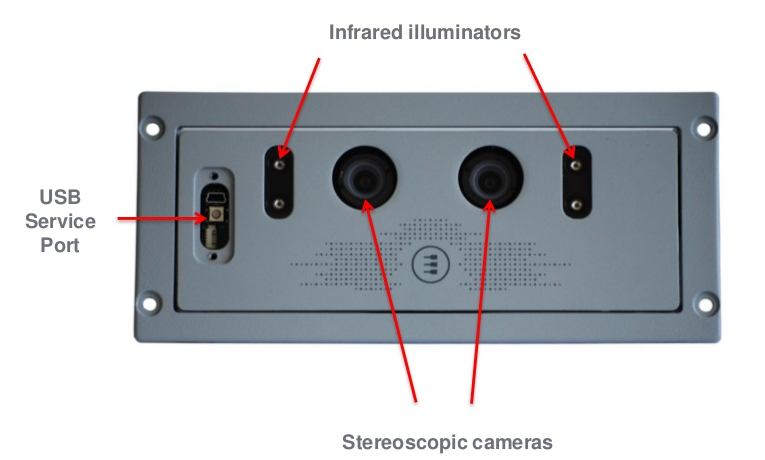
\includegraphics[width=\textwidth]{DispositivoAcquisizioneImmagini.png}
  \centering
  \caption{Dispositivo di acquisizione delle immagini 3D}
  \label{fig:DispAcqImm3D}
\end{figure}

Il dispositivo di acquisizione video visibile in figura \ref{fig:DispAcqImm3D}. Esso nasconde al suo interno una FPGA programmata con una IP proprietaria Eurotech che permette la ricostruzione in 3D delle immagini acquisite dalle telecamere stereoscopiche di cui \`e dotato il dispositivo.
Il funzionamento \`e il seguente: i proiettori di luce infrarosse illuminano la scena, le telecamere a infrarossi stereoscopiche acquisiscono le immagini nello spettro della luce infrarossa. Le due immagini vengono passate alla FPGA che per mezzo di tecniche di ricostruzione stereoscopica accelerate in hardware permette di generare delle immagini in scala di grigi dove l'informazione di profondit\`a \`e data dal colore del pixel. Queste immagini vengono quindi passate all'unit\`a di elaborazione centrale che vi applica un semplice algoritmo per il tracciamento dei passeggeri di cui discuteremo il funzionamento nel dettaglio nel prossimo paragrafo.

%% Interruzione di pagina
\newpage

\subsection{Software}

\begin{figure}[h!]
  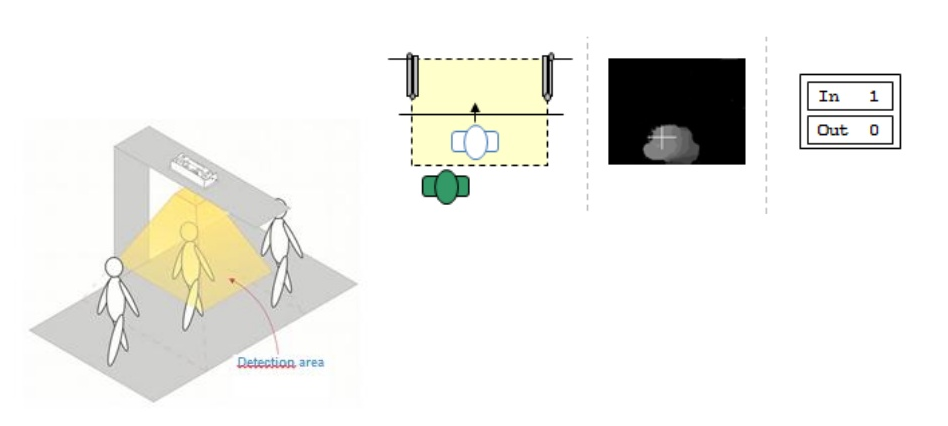
\includegraphics[width=\textwidth]{Algoritmo.png}
  \centering
  \caption{Schematizzazione funzionamento algoritmo tracciamento passeggeri}
  \label{fig:SchemAlgrTrackPCNEurotech}
\end{figure}


\subsection{Problematiche di questa soluzione}


%% Fine dei capitoli normali, inizio dei capitoli-appendice (opzionali)
\appendix

\part{Appendici}

\chapter{Altro capitolo}
Sed purus libero, vestibulum ut nibh vitae, mollis ultricies augue. Pellentesque velit libero, tempor sed pulvinar non, fermentum eu leo. Duis posuere eleifend nulla eget sagittis. Nam laoreet accumsan rutrum. Interdum et malesuada fames ac ante ipsum primis in faucibus. Curabitur eget libero quis leo porttitor vehicula eget nec odio. Proin euismod interdum ligula non ultricies. Maecenas sit amet accumsan sapien.

%% Parte conclusiva del documento; tipicamente per riassunto, bibliografia e/o indice analitico.
\backmatter

%% Riassunto (opzionale)
\summary
Maecenas tempor elit sed arcu commodo, dapibus sagittis leo egestas. Praesent at ultrices urna. Integer et nibh in augue mollis facilisis sit amet eget magna. Fusce at porttitor sapien. Phasellus imperdiet, felis et molestie vulputate, mauris sapien tincidunt justo, in lacinia velit nisi nec ipsum. Duis elementum pharetra lorem, ut pellentesque nulla congue et. Sed eu venenatis tellus, pharetra cursus felis. Sed et luctus nunc. Aenean commodo, neque a aliquam bibendum, mauris augue fringilla justo, et scelerisque odio mi sit amet diam. Nulla at placerat nibh, nec rutrum urna. Donec ut egestas magna. Aliquam erat volutpat. Phasellus vestibulum justo sed purus mattis, vitae lacinia magna viverra. Nulla rutrum diam dui, vel semper mi mattis ac. Vestibulum ante ipsum primis in faucibus orci luctus et ultrices posuere cubilia Curae; Donec id vestibulum lectus, eget tristique est.

%% Bibliografia (opzionale)
\bibliographystyle{plain_\languagename}%% Carica l'omonimo file .bst, dove \languagename � la lingua attiva.
%% Nel caso in cui si usi un file .bib (consigliato)
\bibliography{thud}
%% Nel caso di bibliografia manuale, usare l'environment thebibliography.

%% Per l'indice analitico, usare il pacchetto makeidx (o analogo).

\end{document}

--- Istruzioni per l'aggiunta di nuove lingue ---
Per ogni nuova lingua utilizzata aggiungere nel preambolo il seguente spezzone:
    \addto\captionsitalian{%
        \def\abstractname{Sommario}%
        \def\acknowledgementsname{Ringraziamenti}%
        \def\authorcontactsname{Contatti dell'autore}%
        \def\candidatename{Candidato}%
        \def\chairname{Direttore}%
        \def\conclusionsname{Conclusioni}%
        \def\cosupervisorname{Co-relatore}%
        \def\cosupervisorsname{Co-relatori}%
        \def\cyclename{Ciclo}%
        \def\datename{Anno accademico}%
        \def\indexname{Indice analitico}%
        \def\institutecontactsname{Contatti dell'Istituto}%
        \def\introductionname{Introduzione}%
        \def\prefacename{Prefazione}%
        \def\reviewername{Controrelatore}%
        \def\reviewersname{Controrelatori}%
        %% Anno accademico
        \def\shortdatename{A.A.}%
        \def\summaryname{Riassunto}%
        \def\supervisorname{Relatore}%
        \def\supervisorsname{Relatori}%
        \def\thesisname{Tesi di \expandafter\ifcase\csname thud@target\endcsname Laurea\or Laurea Magistrale\or Dottorato\fi}%
        \def\tutorname{Tutor aziendale%
        \def\tutorsname{Tutor aziendali}%
    }
sostituendo a "italian" (nella 1a riga) il nome della lingua e traducendo le varie voci.
